% Figure 1 panel a: the evolutionary model tested in this study.
% A disease-associated genetic effect reaches fitness twice -- through disease
% liability and through reproduction -- and the sign of the reproductive arm
% decides whether the variation persists.
% Compile: tectonic fig1_panelA_hypotheses.tex
%   -> copy to figures_final/Fig1_panelA_hypotheses.pdf (258 x 156 pt slot)
\documentclass[tikz,border=2pt]{standalone}
\usetikzlibrary{arrows.meta,positioning,calc}
\definecolor{antcol}{HTML}{2C5985}
\definecolor{syncol}{HTML}{C0392B}
\definecolor{srccol}{HTML}{4D4D4D}
\hyphenpenalty=10000 \exhyphenpenalty=10000 \tolerance=9999
\begin{document}
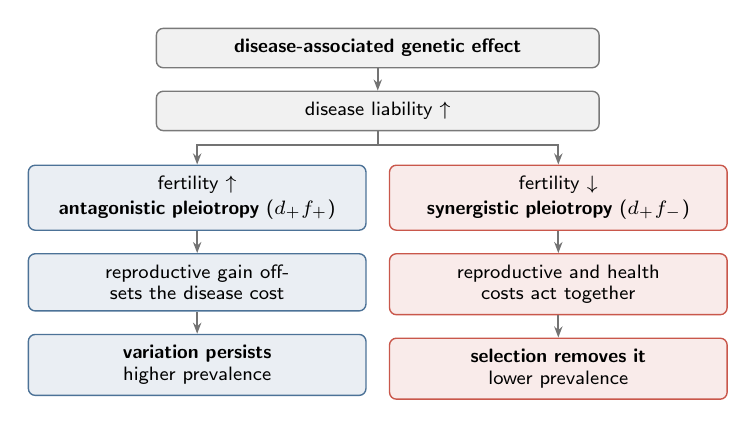
\begin{tikzpicture}[
  font=\sffamily,
  box/.style = {draw, rounded corners=2.5pt, align=center, inner xsep=5pt,
                inner ysep=4pt, line width=0.5pt,
                font=\sffamily\fontsize{6.6}{7.8}\selectfont},
  src/.style = {box, draw=srccol!75, fill=srccol!8,  text width=150pt},
  A/.style   = {box, draw=antcol!85, fill=antcol!10, text width=112pt},
  S/.style   = {box, draw=syncol!85, fill=syncol!10, text width=112pt},
  arr/.style = {-{Stealth[length=4pt]}, line width=0.7pt, black!55}]
\newcommand{\hd}[1]{{\bfseries\fontsize{7.2}{8.4}\selectfont #1}}

\node[src] (g) at (0,0) {\hd{disease-associated genetic effect}};
\node[src, below=8pt of g, text width=150pt] (d) {disease liability $\uparrow$};

\node[A, below left=12pt and 4pt of d.south, anchor=north east] (a1)
  {fertility $\uparrow$\\[1pt]\hd{antagonistic pleiotropy} ($d_{+}f_{+}$)};
\node[S, below right=12pt and 4pt of d.south, anchor=north west] (s1)
  {fertility $\downarrow$\\[1pt]\hd{synergistic pleiotropy} ($d_{+}f_{-}$)};

\node[A, below=8pt of a1] (a2) {reproductive gain offsets the disease cost};
\node[S, below=8pt of s1] (s2) {reproductive and health costs act together};

\node[A, below=8pt of a2] (a3) {\hd{variation persists}\\ higher prevalence};
\node[S, below=8pt of s2] (s3) {\hd{selection removes it}\\ lower prevalence};

\draw[arr] (g) -- (d);
\draw[arr] (d.south) -- ++(0,-5pt) -| (a1.north);
\draw[arr] (d.south) -- ++(0,-5pt) -| (s1.north);
\draw[arr] (a1) -- (a2); \draw[arr] (a2) -- (a3);
\draw[arr] (s1) -- (s2); \draw[arr] (s2) -- (s3);
\end{tikzpicture}
\end{document}
